%!TEX TS-program = xelatex
%!TEX encoding = UTF-8 Unicode

\documentclass[11pt,tikz,border=1]{standalone}

\begin{document}
  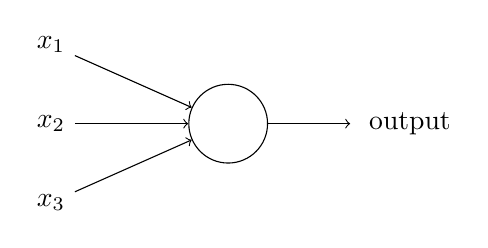
\begin{tikzpicture}[
    neuron/.style={circle,draw,inner sep=0pt,minimum size=10mm}
    ]

    \node (perceptron) at (0, 0) [neuron] {};
    \node (output) at (2.25, 0) {\ output};
    \node (x1) at (-2.25, 1) {$x_1$};
    \node (x2) at (-2.25, 0) {$x_2$};
    \node (x3) at (-2.25, -1) {$x_3$};
    \draw [->] (x1) to (perceptron);
    \draw [->] (x2) to (perceptron);
    \draw [->] (x3) to (perceptron);
    \draw [->] (perceptron) to (output);

  \end{tikzpicture} 
\end{document}
